%
%--------------------------------------------%
% Packages arranged by : Tsz Timmy Chan	     %
%                 Date : June 12th, 2019     %
%--------------------------------------------%

\documentclass{TC}
\usepackage{TCcommon}

\title{Learning Trajectories and Progressions}	% Work Title Here.
\author{Tsz Timmy Chan}	% YOUR NAME HERE 


\usepackage[style=numeric]{biblatex}
\addbibresource{LS.bib}


\usepackage[notes]{TCheader}
\usepackage{TCexamtitle}
%\renewcommand{\benediction}{" " - }
%\renewcommand{\quoteoftheday}{" " \\ - }
\begin{document}
\subsubsection{Learning Trajectories and Progressions}
In order to give a proper definition of learning trajectories and progressions, we must first begin with preliminary definitions.

Given an academic discipline, there exist ways to describe the paths to student growth and mastery. Researchers and teachers conduct this theoretical work with variety of intentions and focus, leading to a corniucopia of styles and approaches to the study and creation of learning trajectories and progressions. In  \parencite{duncan_learning_2018}, Duncan and Rivet give a general definition of \gls{ltp}. In \parencite{lobato_taxonomy_2017}, Lobato and Walters give a detailed description of seven different types of intentions/perspective on \gls{ltp}. 
 
First, knowledge in an academic field beckons organization, and the first operation we do is to separate out knowledge into \emph{constructs}, which are defined as follows:

\begin{mdframed}
\begin{definition}[Construct]
\emph{Constructs} are large ideas in an academic discipline, usually defined in a way to partition a subject in order to understand cognition and learning. One can consider this defining subsets of the knowledge of a discipline.  \end{definition}
\end{mdframed}

Note that constructs are subjectively defined, and the ways they are defined reveal the researcher's intention. Furthermore, constructs may contain other constructs; I.e., If $A$ is some construct, then there may exist $A_1, A_2, \ldots, A_n \subset A$. Note that in this description, we consider finite $n$, as most applications of hypothetical models of learning in the form \gls{ltp} contain finitely many constructs.

\begin{example}
Suppose we have a topic $A = \text{"Functions in Precalculus"}$, and we wish to use a disciplinary-logic approach (defined in \ref{disciplinary_logic}) to describe a set of constructs that may be defined using skills and definitions. For a rudimentary example:
\begin{align*}
A_1 &= \text{"Use of variables"},\;A_2 = \text{"Mapping / Relations"},\\
A_3 &= \text{"Graphs of equations in } \R^2 \text{"},\;A_4 = \text{"One to one"},\\
A_5 &= \text{"Inverse functions"}, \cdots \\
\text{by construction: }& A_1, \cdots, A_5 \subset A
\end{align*} 
\end{example}
Note here that for some arbitrary $i,j$, $A_i \cap A_j \stackrel{?}{=} \emptyset$. 
\begin{mdframed}
\begin{definition}[Pathway between constructs]
A pathway between constructs shows a connection between ideas, usually for pedagogical reasons or disciplinary expertise. A pathway between constructs may contain intermediate steps, with a diverse set of pathways. 
\end{definition}
\end{mdframed}

\begin{remark}
I wonder if creating \gls{ltp} with disjoint constructs is useful or not? Or acknowledging the overlaps can create better "knowledge webs"? Can one define the pathways and the constructs the edges and nodes of knowledge countable? discrete?
\end{remark}
 
 In essence, once constructs are separated out and defined using some rule (this may be based on education research or academic expertise), one is imposing some partial order on these constructs, where the this order may be defined in multiple ways, depending on the academic field.
 
 \begin{mdframed}
\begin{definition}[Learning trajectories and progression]
A \emph{learning trajectory} (LT) or \emph{learning progression} (LP) is a hypothetical model used describe student growth and mastery in an academic subject, usually with intermediate \emph{levels} and \emph{pathways}. Usually, mathematics educators use "trajectories" and science educators use "progressions". We call a \gls{ltp} \emph{linear} when the \gls{ltp} models a \emph{well ordered set}.
\end{definition}
\end{mdframed}
\subsubsection{Common Properties of \gls{ltp}}

As researchers have finite time and resources, one must define a limitation on the scope of an \gls{ltp}:

\begin{mdframed}
\begin{definition}[Scope of \gls{ltp}]
\gls{ltp} have a defined \emph{scope}, which consists of
\begin{itemize}
\item a particular slice of knowledge (domain of study), \item and a specific age-group (span).
\end{itemize}
Conventionally, the starting point of an \gls{ltp} is called the \emph{lower anchor}, represented with a beginner or novice level of understanding within the scope, and the ending point of an \gls{ltp} is called the \emph{upper anchor}, which represents the proficiency level within the scope.
\end{definition}
\end{mdframed}
\gls{ltp}, by its nature, describe student mastery and progress over a given scope. Naturally, this gives rise to another component of \gls{ltp}:
\begin{mdframed}
\begin{definition}[Levels of \gls{ltp}]
A \gls{ltp} usually contain definitions of levels, which are types of construct that are categorized by \parencite{duncan_learning_2018} \parencite{lobato_taxonomy_2017}:
\begin{enumerate}[(i)]
\item Content ideas or cognative conceptions, \label{levels_content}
\item Practice and discourse patterns \label{levels_practice_and_discourse}
\item A mix of \ref{levels_content} and \ref{levels_practice_and_discourse} 
\item Observable strategies
\item Textbook tasks
\end{enumerate}
\end{definition}
\end{mdframed}

A way to study and compare two different \gls{ltp} in the same field is to consider how many constructs are spread over a particular length of time. This gives rise to the following definition:

\begin{mdframed}
\begin{definition}[Grain Size of \gls{ltp}]
The "size" of the jump between each level or construct. Usually can be viewed the following: Let $c$ be the number of constructs, and $t$ be the amount of time in the scope of the LT. Then the grain size is defined as $g = \displaystyle \frac{c}{t}$. Furthermore, given $g_1 , g_2$ are two grain sizes, suppose $g_1 < g_2$, then we say $g_1$ is "coarser" and $g_2$ is "finer". (This is the same language as the descriptors for the partition of an interval.)
\end{definition}
\end{mdframed}
 \begin{remark}The grain-size and the number of paths given differ based on the intention of the researcher as well as the targeted audience.  \end{remark}

Given that \gls{ltp} describe "growth", this implies that there is some order that can be imposed on the models of student mastery over knowledge, either in terms of content, dialogue or both. Thus, the language of partially ordered sets is appropriate here, where each level or construct is an element, and the pathways between the levels is an edge or order relation. Thus \gls{ltp} may be considered as a directed graph. 

Since \gls{ltp} describe growth from point $A$ to point $B$, we may impose an \emph{order} on the set of knowledge, once constructs and levels are defined. Some common types of ways to characterize and measure "progress" \parencite{duncan_learning_2018}: 
\begin{mdframed}
\begin{definition}[Individual progress along a \gls{ltp}]
Individual progress can be defined as "major re-conceptualizations of knowledge and beliefs because students' na\"ive understandings are often incommensurate with canonical scientific ideas." - Idea is that students have a network of knowledge that becomes better approximations of the expert knowledge as students progress along the levels.
\end{definition}
\end{mdframed}

Individual progress has been the center of study for most subjects, while in mathematics education there's been another perspective on viewing progress:

\begin{mdframed}
\begin{definition}[Community progress along a \gls{ltp}]
Communal progress can be measured as changes in the discourse and practice from the community perspective. Duncan cites Cobb and colleagues \gls{ltp}, which "captures the changes in classroom norms and mathematical practices." Tasks and tools to help achieve the goal of community learning are often included. 
\end{definition}
\end{mdframed}
\begin{remark}
Given a particular discipline, (the pure mathematician in me asks) can we partition a given scope into infinitely many levels, with \gls{ltp} that has infinitely-fine grain size? Perhaps this is the difficulty;t we're using discrete abstractions that hope to closely model the learning process from the instructor or the student perspective, while the experience of learning is one of flow and students experience learning as a continuum of experiences.
\end{remark}

\subsubsection{Claims about \gls{ltp}}
While the constructs is connected to many paths, there seems to be a boundary in which these paths can be drawn effectively. While the number of paths may be infinite, the area which they cover are not. Effective models of descriptive paths is an optimization problem, where there exists finite amount of space and time to describe paths between constructs; and at best, we have some hypothetical model to describe the space of paths between two constructs. These educated conjectures based on research that must be continued to be refined.

\begin{conjecture}[Directed graph conceptualization of \gls{ltp}]
Suppose we impose some order (type of progression) and define constructs associated with the order. Then suppose $A<B$ in some \gls{ltp}. First, there exists at least one path between $A$ and $B$, and there \emph{likely} exists intermediate constructs or levels $\{C_1, C_2, \cdots, C_k\}$. We then define the vertex set to be $\{A, B, C_1, \ldots,C_k\}$ and edges as the pathways between these constructs. This give rise to finitely many paths due to the constraints described above. 
\end{conjecture}

\begin{remark}
Math nerd side note: An \gls{ltp} with this must be some sub-graph of the complete $(k+2)$-directed-graph. This means that the number of pathways, or edges, in an \gls{ltp} with $k$ constructs connecting $A$ and $B$ has the following bounds:

$$ k+ 1 < \text{(Number of pathways)} < 2\sum_{n=0}^{k+1}n = (k+1)(k+2)$$ 

\end{remark}

This way of describing \gls{ltp} gives rise to two quick corollaries:

\begin{corollary}
 \gls{ltp} are not necessarily linear.
\begin{proof}Given we use the language of posets and directed graphs, this is a linear \gls{ltp} is a special case of the general \gls{ltp}. Literature review reveals that "learning is multi-dimensional, context-dependent and therefore likely not linear" \parencite{duncan_learning_2018}\end{proof}
\end{corollary}

\begin{corollary}
A \gls{ltp} may contain cycles.

\begin{proof}In these models, we have directed graphs to indicate progress in maturity of dialogue or to record technical dependencies. Then note that the directed graph that models a particular \gls{ltp} may contain cycles. Duncan and Rivet \parencite{duncan_learning_2018} referred to Battista's research, that students may use more rudimentary ways of reasoning when tackling more complex questions, even though they may have shown proficiency in more sophisticated techniques.
%TODO cite Battista%
 \end{proof}
\end{corollary}
\subsubsection{Development and Refinement of \gls{ltp}}
\gls{ltp} are by definition hypothetical constructs, and their development involves a few usual phases, similar to the engineering design cycle:

\begin{enumerate}[(1)]
\item\label{lit_review} A well formed hypothesis usually begins with a throughout literature review: 
	\begin{enumerate} 
	\item if \ref{lit_review} yields sufficient existing research: design a well-specified \gls{ltp} and go to refinement.
	\item else, use these following techniques \parencite{duncan_learning_2018}:
		\begin{itemize}
		\item Assessment-driven cross-sectional studies of student thinking using interviews and written assessments.
			\begin{itemize}
			\item[Pro:] When interviews are done under status quo setting, the study has the benefit of reflecting what students can do under less than ideal learning environments. Written-assessments\footnote{Commonly used statistical models: Rasch models, latent class analyses, Bayesian networks)} are used to help scale to larger sample of students.
			\item[Con:] Written assessments are difficult to design, especially to elicit responses that can demonstrate the full range of the progression. Optimization problem between the number of assessments and the discrete nature of assessments in a continuum of learning.
			\end{itemize}
		\item short and long (i.e., longitudinal) teaching experiments using design-based research to characterize the development of students' ideas under specified instructional conditions
			\begin{itemize}
			\item[Pro:] Development of instructional interventions modified based on observed student performance allows for a more grass-roots, bottom up approach to validating \gls{ltp}. 
			\item[Con:] \gls{ltp} that is written and designed for a specific condition leads to a question of whether generalizing this is easy. \textbf{Open research question:} Whether learning paths would look different under dissimilar instructional conditions is unknown.
			\end{itemize}
		\end{itemize}
	\end{enumerate}
\end{enumerate}

\subsubsection{Seven approaches to \gls{ltp}}
Lobato and Walters \parencite{lobato_taxonomy_2017} gave a detailed taxonomy of approaches to \gls{ltp} in state-of-the-art research. In their taxonomy, they classify the different approaches into seven categories; however, note that a given \gls{ltp} may be born of a melange of a few perspectives.

\subsubsection{Cognitive levels}

In the cognitive levels perspective, cognitive milestones are ranked in order of sophistication but hierarchies may be weak or strong. Similar to the language used in mathematical induction, strong assumes all steps before are mastered. Mostly linear in nature, but students may enter at a variety of levels and may fall back or climb forward. 
\begin{multicols}{2}
\begin{itemize}
\item Features: Levels or constructs may be organized using mental actions, fine-grained progression or clustering meanings by observing different types of abstraction. For \gls{ltp} written in this approach, emphasis is placed on the quality of the narrative, or group discussions rather than the content.

\item Methods: Created using cross-sectional interviews over multiple grade levels. 

\item Purpose: Diagnostic assessment

\item Benefits: In the example cited by Lobato and Walters, Teachers can access reports of their students' thinking, given that assessments are written to associate particular responses with facets, giving rise to facet-driven instructional resources.

\item Trade-offs: Learning mechanisms on how students morph their understanding by shaping their thoughts from one level to the next is hidden. Progression of understanding of innovative teaching techniques is limited. Important scientific habits of explaining or conjecturing is not emphasized. 
 \end{itemize}
 \end{multicols}
 
\subsubsection{Levels of discourse}

Progress is described as increasingly sophisicated ways of communicating in use of language, of thinking and of acting. Lower anchor is the informal primary discourse. This type of \gls{ltp} tends to have coarser grain size.

\begin{multicols}{2}
\begin{itemize} 
\item Features: Progress along levels of discourse has been defined in a variety of ways. Levels might represent using secondary discourse. Some use Toulmin's \footnote{Who is Toulmin?} model of argumentation.
\item Methods: Constructed and evaluated using written data collected across multiple grade levels, as well as an example of research inside the classroom to account for differences in instruction. 
\item Purpose: "Literacy is characterized as the mastery of a particular discourse that is acquired through increased participation in communities where that discourse is common and valued." 
\item Benefits: This research provides a tool by which instruction can be aligned with state standards. 
\item Trade-offs: This is currently more biased towards science education than mathematics education researchers. 
 \end{itemize}
 \end{multicols}
 
 
\subsubsection{Schemes and operations}

 Generate a model of students' initial schemes and mental operations and infer the modifications of students' schemes over time, where schemes are defined by Piaget. Piaget is famous for the stages of development in cogitative science.
\begin{mdframed}
\begin{definition}[Scheme]
% TODO: citation?
A scheme is conceived as a researcher's construct used to model students' concepts.
According to von Glasersfeld, a scheme consists of three parts
\begin{enumerate}[(1)]
\item Trigger conditions - Set of internal conditions, such that when satisfied will activate the scheme;
\item way of operating mentally and physically;
\item anticipation of the outcome of the activity.
\end{enumerate}
According to Norton and McCloskey (2008), schemes are activated holistically rather than sequentially like a strategy. 
\end{definition}
\end{mdframed}


\begin{multicols}{2}
\begin{itemize}
\item Features: In an demonstrative example, the centerpiece of the trajectory is the construction and evolution of schemes. Focus tends to be on mental operations, with an emphasis on student's mental coordination and reflective abstraction. Less variety because of the shared theoretical perspective of "Piagetian constructivism." Common assumption is that students respond to particular activities and instruction based on their current conceptual structures.
\item Methods: Teaching experiment where research-teacher working in parallel.
\item Purpose: Micro-analysis of the evolution of individual understanding, with a focus on students' learning rather than the logic of a mature mathematician
\item Benefits: Provides useful constructs to other researchers
\item Trade-offs: Small $n$ limits researchers ability to generalize, and $\exists$ few efforts to extend this approach by codifying the instructional moves that support the construction of students' ideas.
 \end{itemize}
 \end{multicols} 
  
\begin{remark}
What is the difference between schemes and schema which is "a cohesive, repeatable action sequence possessing component actions that are tightly interconnected and governed by a core meaning."?
\end{remark}
\subsubsection{Hypothetical learning trajectories} 

 Captures the ways teachers posits a conjecture regarding their students' current understanding and develops activities that they think will support their students in constructing more sophisticated ways of reasoning. This approach commonly consists of three components: learning goal, levels of thinking, instructional tasks.
 
\begin{multicols}{2}
\begin{itemize}
\item Features: Ongoing modification of \gls{ltp}, "to offer a conceptualization of teaching as being informed by a constructionist perspective on learning."
\item Methods: Data on students' initial concepts is collected using interviews + assessments.
\item Purpose: Used mainly as teaching resource, and is very dynamic. Instructional tasks aim to inspire and help students to reach the next level of sophistication in their learning.
\item Benefits: (Perhaps) a good tool for improving mathematics instruction. 
\item Trade-offs: Goals focused on standards documents, so \gls{ltp} do not speak to what is possible when teachers focus on mathematical goals not in the standards.
 \end{itemize}
 \end{multicols}
 
\subsubsection{Collective mathematical practices}

 Focus on \emph{emergent perspective} which :individual constructs are coordinated with collective constructs, such as social norms and classroom practices."
 
 \begin{remark}
  In an ancestral way, each class is a different community, and has a different norm for communicating. Personally, I've observed this while teaching precalculus courses in a few semester at SFSU.
 \end{remark}
\begin{multicols}{2}
\begin{itemize}
\item Features: Researchers have begun with observable actions/strategies, and progressed towards observing what can function "as-if-shared" in the framework of cognitive sciences. The communal nature of the description of levels  causes most of this type of \gls{ltp} to also include descriptions of collective constructs such as social norms and sociomathematical norms.
\item Methods: Documenting Collective Activity (DCA) method, a three phased method:
\begin{enumerate}[(i)]
\item generate a log of student argumentation and record structure of statements
\item record when students accept a previously disputed claim as truth or when a previous claim/conjecture becomes supporting data in another argument, or when an idea is repeatedly used as data.
\item researchers then cluster mathematically related, normative ways of reasoning and provide a \gls{ltp}
\end{enumerate}

\item Purpose: inform "instructional theory and design" 
\item Benefits: Embraces the way teachers experience a classroom - as a community.
\item Trade-offs: In order to have discussions, the class social norms must be conducive to student sharing before argumentation can occur.
 \end{itemize}
 \end{multicols}
 
 
\subsubsection{Disciplinary logic and curricular coherence}\label{disciplinary_logic}

 Generated and reflected upon experts' knowledge of the domain, synthesizing research from studies of student knowledge and learning. Structure of the disciplinary knowledge is strongly emphasized, and provides a macro view of how student proficiency in a domain may develop over a long span of time. 
 
\begin{multicols}{2}
\begin{itemize} 
\item Features: "Most make explicit the intertwining of content and inquiry-oriented practices." Because of their intended audience and purpose, all \gls{ltp} written from this approach will contain "learning performances and assessment tasks aligned with the progressions."
\item Methods: Existing research and discipline logic inspire these types \gls{ltp}.
\item Purpose: Inform curricular organization and textbook content towards coherency and cohesion. Provides "horizon knowledge" for teachers. 
\item Benefits: Accessible for a wide audience!
\item Trade-offs: Lack consistency due to drawing from a large variety of research conducted with different goals/settings; trajectories aligned with standards are inflexible and limit growth. These types of \gls{ltp} can be very skill focused.  
 \end{itemize}
 \end{multicols}

\begin{figure}[h]
\centering
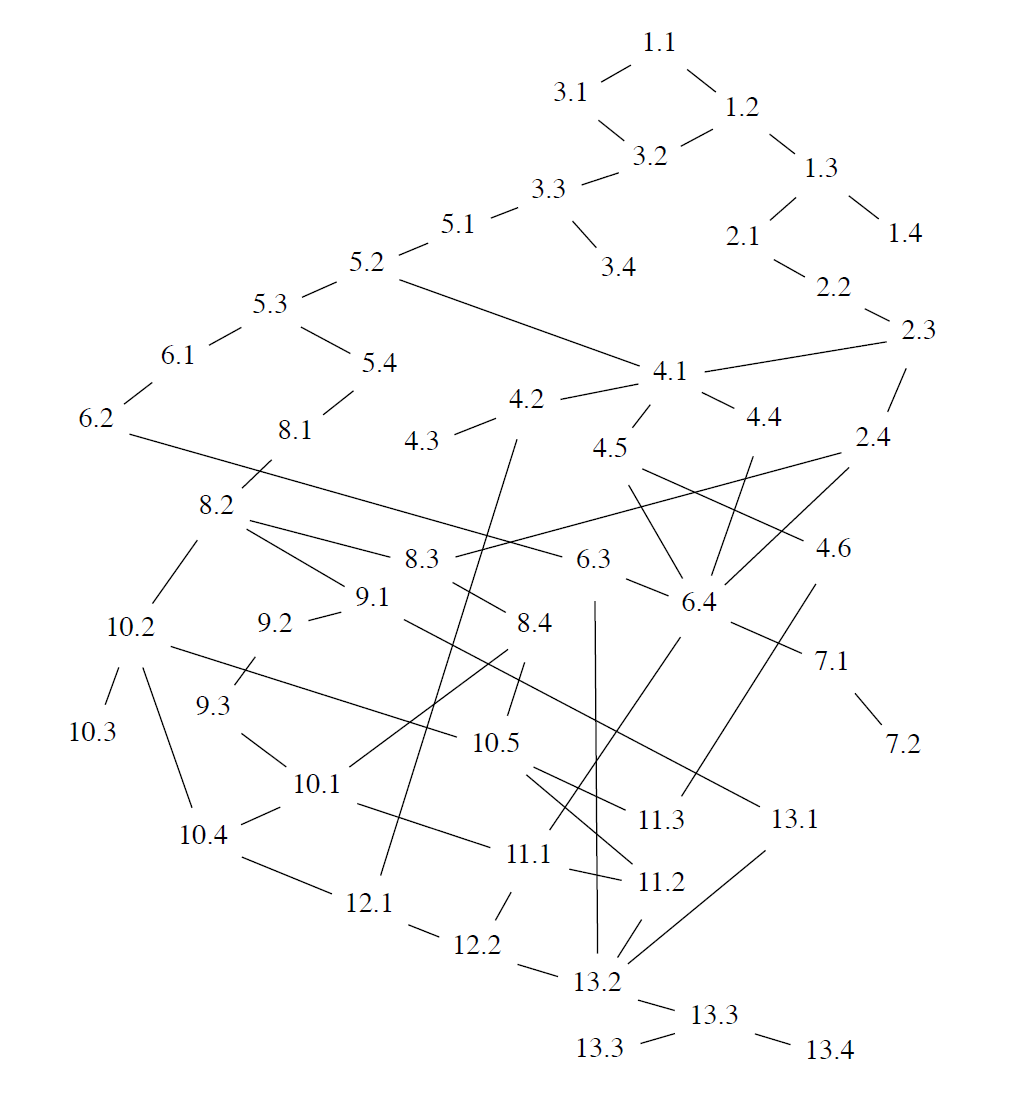
\includegraphics[width=.6\textwidth]{AoP_poset_of_section_dependencies} 
 \caption{"The partially ordered set of section dependencies" \parencite{beck_computing_2016}
\label{disciplinary_logic_LT_example}}
 \end{figure}
  
\begin{remark} Figure \ref{disciplinary_logic_LT_example} is an example that is self-contained and was not intended as an \gls{ltp} (since it was presented without instructional guides). Since the image is from a book on proofs meant to describe the logical, mathematical dependencies, this is genuinely a technical extreme version of a disciplinary-logic-and-cirricular-coherence approach to \gls{ltp}. \end{remark}

 
\subsubsection{Observable strategies and learning performances}
 
  Progress is described using observable behaviors, strategies or other learning performances, and each level is described using action verbs instead of mental conceptions.
  
\begin{multicols}{2}
\begin{itemize}
\item Features: Levels are organized using observable strategies or behaviors. There are differing assumptions in examples of \gls{ltp} written in this perspective about the connections between cognition and behavior.
\item Methods: Could be a product of research or informed by research.
\item Purpose: Communicating with teachers and teacher professional development. 
\item Benefits: Increase the precision and explicitness of \gls{ltp}, and help provide diagnostic or formative assessment information to teachers.
\item Trade-offs: Can miss out on details about conception/cognition. 
 \end{itemize}
 \end{multicols}
 
\subsubsection{Critiques of \gls{ltp} Research}

Diagnosing students and placing them in the appropriate level in an \gls{ltp} is not trivial. There are students who may appear to be on two different levels at the same time. Currently, the research in \gls{ltp} do adequately address the pressing issues of equity, diversity, race, language.

\end{document}